\documentclass[11pt,a4paper]{article}

\usepackage[T1]{fontenc}
\usepackage[utf8]{inputenc}
\usepackage{lmodern}
\usepackage[margin=2.4cm]{geometry}
\usepackage{amsmath,amssymb,amsthm}
\usepackage{booktabs}
\usepackage{tabularx}
\usepackage{array}
\usepackage{xcolor}
\usepackage{listings}
\usepackage{enumitem}
\usepackage{microtype}
\usepackage[ruled,vlined,linesnumbered]{algorithm2e}
\usepackage{tikz}
\usetikzlibrary{arrows.meta,positioning}
\usepackage[hidelinks]{hyperref}

\definecolor{codebg}{gray}{0.95}
\lstset{basicstyle=\ttfamily\small, backgroundcolor=\color{codebg}, breaklines=true,
        columns=fullflexible, frame=none, xleftmargin=0.5em, aboveskip=0.6em, belowskip=0.6em,
        keepspaces=true, showstringspaces=false}

\newcommand{\code}[1]{\texttt{#1}}
\newcommand{\R}{\mathbb{R}}
\newcommand{\E}{\mathbb{E}}
\DeclareMathOperator{\clip}{clip}
\DeclareMathOperator{\rank}{rank}
\DeclareMathOperator*{\argmin}{arg\,min}
\newtheorem{proposition}{Proposition}
\setlength{\emergencystretch}{3em}

\title{A Low-Turnover, Volatility-Budgeted Trading Agent\\for the ACM ICAIF 2026 Trading Agent Competition\\[0.4em]
\large Implementation, methodology, evidence and reproduction guide}
\author{Team \emph{alexleaves}}
\date{6 October 2026 \quad (production configuration version \code{2026-10-06.1})}

\begin{document}
\maketitle

\begin{abstract}
\noindent
This document specifies the trading agent submitted by team \emph{alexleaves} to Competition~99 (ACM ICAIF 2026
Trading Agent Competition). The agent allocates across the fixed 30-stock universe seven times per trading day.
Its live decisions come from a single, deliberately simple rule (\emph{approach~1}). It holds an equally weighted
long-only stock book whose total size (the \emph{exposure}) targets an annualised volatility of 10\% within
$[0.5,0.8]$; the remainder stays in cash. It rebalances only when holdings drift outside no-trade bands.
Two further approaches were implemented and evaluated: a pooled LightGBM cross-sectional return model
(\emph{approach~2}) and an online exponentially weighted blend of alpha ``experts'' (\emph{approach~4}). Both
showed a small, real predictive signal but did not improve competition outcomes after the 0.1\% transaction fee,
so they run in \emph{shadow mode}: they are computed and logged every round but never traded. We describe the competition
mechanics that motivate this design, all mathematical components, the data pipeline, the backtesting and selection
methodology, the results, the live execution system, the test suite, and a step-by-step procedure that lets a third
party regenerate every dataset, trained model, experiment table and live decision.
\end{abstract}

\tableofcontents
\newpage

%=====================================================================
\section{Overview}
%=====================================================================

\paragraph{What the agent does.} At each decision round the agent:
\begin{enumerate}[nosep]
  \item downloads the latest completed hourly bars for the 30 stocks from Yahoo Finance and validates their freshness;
  \item estimates the volatility of an equally weighted portfolio from the last 126 completed trading days;
  \item sets the stock exposure $e=\clip(0.10/\hat\sigma,\,0.5,\,0.8)$ and the target $w^\star_i=e/30$ for every stock;
  \item compares $w^\star$ with the current portfolio weights and uploads a new target \emph{only} if the deviation
        exceeds the no-trade bands ($\|w^\star-w\|_1>0.20$ or $\|w^\star-w\|_\infty>0.05$); otherwise it uploads nothing,
        which under the competition rules keeps the current holdings at zero cost.
\end{enumerate}
Approaches~2 and~4 compute alternative \emph{tilted} targets every round; these are written to the decision log
for later comparison but are not traded.

\paragraph{Headline evidence.} Over 224 historical 15-trading-day windows (official data, 2021--2025) and 115 windows
(Yahoo data, mid-2024 to October 2026), each simulated exactly like the Official phase, the production configuration
finished on average 2.46th and 2.38th respectively among 17 strategies (itself plus a field of 16 simple competitor
strategies). It made about one trade per window, with mean turnover $\approx0.007$. Its average position stayed between 2.15 and 2.81 in
every calendar year, including the 2022 bear market. It stayed within $[2.30,2.48]$ under every parameter perturbation tested.

%=====================================================================
\section{Competition rules and what they imply}\label{sec:rules}
%=====================================================================

\subsection{Rules reproduced by the agent and the simulator}
The following rules come from the official starter kit (\code{docs/rules.md}, \code{docs/evaluation.md}) and the live
schedule served by the organiser backend:
\begin{itemize}[nosep]
  \item Universe: 30 U.S.\ equities in six sectors of five (\code{universe.json}).
  \item Each phase starts with USD 1{,}000{,}000 in cash in an independent account. Validation runs 8--9 October 2026
        (14 rounds); Official runs 12--30 October 2026 (15 days, $K=105$ rounds).
  \item Seven rounds per day execute at 09:30, 10:30, \dots, 15:30 ET. Upload deadlines are 09:10 and then five minutes
        before each later execution. A window opens 10 minutes after the previous execution (Round~1 opens at 15:40 ET
        on the previous trading day).
  \item A decision is a vector of target weights $w\in\R^{30}$ with $0\le w_i\le0.30$ and $\sum_i w_i\le1$; the
        remainder is cash. Long-only, no leverage, fractional shares.
  \item Each rebalance pays a fee of $\phi=0.1\%$ of total buy-plus-sell notional, including the initial allocation.
  \item The first upload in a window consumes the round. A missing (or invalid) decision \emph{holds} the portfolio with
        zero traded notional.
\end{itemize}

\subsection{Evaluation metrics}
Order non-cancelled rounds $k=1,\dots,K$. Let $B_k$ be the NAV immediately before round $k$ executes, $E_k=B_{k+1}$ the
NAV at the end of its period, $E_K$ the final official close, $N_k$ the round's buy-plus-sell notional, and
$r_k=E_k/B_k-1$. The four metrics are
\begin{align}
  M_1 &= \frac{E_K}{B_1}-1, &
  M_2 &= \sqrt{1764}\,\frac{\bar r}{s_r}, \\
  M_3 &= \max_{1\le m\le L}\frac{P_m-V_m}{P_m},\quad P_m=\max_{j\le m}V_j, &
  M_4 &= \frac1K\sum_{k=1}^K\frac{N_k}{B_k},
\end{align}
where $s_r$ is the sample standard deviation of $r_k$ and $V_0,\dots,V_L$ is the chronological sequence of the initial NAV,
every period endpoint and every daily 16:00 close. Teams are ranked on each metric (higher $M_1,M_2$; lower $M_3,M_4$),
ties receive average ranks, and the \emph{overall rank score} is the mean of the four ranks (lower is better).

\subsection{Implications for strategy design}\label{sec:implications}

\begin{proposition}[Exposure scaling]\label{prop:scaling}
Let a strategy hold a fraction $e\in(0,1]$ of NAV in a fixed-composition stock portfolio with period returns $\rho_k$,
and the rest in zero-return cash. Ignoring fees, $r_k=e\rho_k$. Hence $M_2$ does not depend on $e$, $M_1\approx e\,M_1(1)$
to first order, $M_3\approx e\,M_3(1)$ to first order, and the initial allocation alone contributes $e/K$ to $M_4$.
\end{proposition}
\noindent
Thus, relative to fully invested competitors, lowering exposure improves two ranks ($M_3$, $M_4$), leaves one
unchanged ($M_2$) and worsens one ($M_1$) only when markets rise. The optimal exposure is a property of the field of
competitors, not of the market alone (Section~\ref{sec:choice}).

\paragraph{Fees against predictability (back-of-envelope).}
Let an active, dollar-neutral tilt $a=A\,z/\|z\|_1$ follow standardised signal scores $z$ whose rank correlation
(information coefficient, IC) with next-day relative returns is $\rho$. Let the cross-sectional standard deviation of
daily returns be $\sigma_x$. For roughly Gaussian $z$ with $N=30$, $\|z\|_2^2/\|z\|_1\approx\sqrt{\pi/2}$, so the
expected daily active return is approximately
\begin{equation}
  \E[a^\top r]\;\approx\;\sqrt{\pi/2}\;\rho\,\sigma_x\,A .
\end{equation}
If the signal renews daily, the active book turns over roughly $A$ per day at cost $\phi A$. In our data
$\sigma_x\approx1.65\%$ (mean over 2021--2025), so break-even requires $\rho\gtrsim\phi/(\sqrt{\pi/2}\,\sigma_x)\approx0.048$.
The best model we trained has out-of-sample IC between $0.006$ and $0.029$ (Table~\ref{tab:ic}). We therefore expect,
and observe, that trading on such signals destroys value unless turnover is suppressed so heavily that the tilt is
almost never traded.

%=====================================================================
\section{Data}\label{sec:data}
%=====================================================================

\subsection{Official development dataset}
The organisers publish hourly OHLCV bars for the 30 stocks from 4 January 2021 to 31 December 2025 as Codabench dataset
1833 (\code{hourly\_market\_data\_2021\_2026.zip}, SHA-256
\code{396a36e8\ldots51652}, 263{,}001 rows, one Parquet file). Bars are timestamped at their \emph{start} in naive
U.S./Eastern time and are clock-aligned: 09:30--10:00, 10:00--11:00, \dots, 15:00--16:00. The pipeline
(\code{bot/data.py}) verifies the checksum and applies three corrections:
\begin{enumerate}[nosep]
  \item \textbf{Early closes.} On the ten NYSE 13:00 early-close days, 520 thin after-hours rows (bars after 13:00) are
        removed. The 13:00 bar, which carries the closing auction, is kept.
  \item \textbf{Outages.} On five days (2021-04-19, 2021-10-25, 2022-01-24, 2022-01-26, 2022-03-08) most bars are
        missing. The data is placed on a complete (session bar $\times$ ticker) grid; 469 missing bars are filled flat
        from the previous close with zero volume and flagged.
  \item \textbf{Spinoffs.} Prices are split-adjusted but not adjusted for spinoffs, which appear as spurious overnight
        losses. With pre/post value ratios $f$ (GE 2023-01-04: 1.281; GE 2024-04-02: 1.253; T 2022-04-11: 1.324), each
        price before a spinoff is divided by the product of all later factors of that ticker:
        $\tilde P_t=P_t\big/\prod_{s>t}f_s$.
\end{enumerate}
Prices are not dividend-adjusted. This has negligible effect on volatility estimates and does not affect
cross-sectional features beyond dividend days.

\subsection{Yahoo Finance data}
The live agent reads Yahoo Finance through \code{yfinance} (hourly bars, \code{prepost=False}, unadjusted for
dividends). Yahoo hourly bars start on the half hour: 09:30--10:30, \dots, 14:30--15:30, 15:30--16:00. They therefore
coincide exactly with the competition execution times, which is not true of the official bars. Hourly history is
limited to about 730 days (the cached file starts on 2023-11-08; the first week, which lacks some tickers, is trimmed,
so the panel starts on 2023-11-15). Daily bars since 2021 are also cached for cross-checks. Bars that have not finished
at download time are discarded.

\paragraph{Cross-source agreement.} After spinoff back-adjustment, daily closes built from the official bars agree with
Yahoo daily closes to a median absolute difference of 0.017\% (99th percentile 0.149\%) over 1{,}255 days. Only 58
ticker-days differ by more than 0.5\%, almost all on the outage days above.

\subsection{Bar timing}\label{sec:bartiming}
Let a day's bars start at $s_1<\dots<s_m$. Bar $j<m$ ends at $s_{j+1}$. The last bar ends at the session close
$c=$ 13:00 if $s_m<$ 15:00 (early close) and 16:00 otherwise (\code{bot/market.py}, \code{bar\_end\_times}). A bar is
\emph{available} at time $t$ if its end is $\le t$. The execution price at time $\tau$ is the open of a bar starting at
$\tau$ if one exists (always true for Yahoo bars). Otherwise it is the midpoint $(O+C)/2$ of the bar containing $\tau$; this
approximation is used only for the 10:30--15:30 executions on the clock-aligned official data.

%=====================================================================
\section{Decision timeline and information sets}
%=====================================================================

For round $k$ with execution time $\tau_k$, the upload window opens at $o_k=\tau_{k-1}+10$ min, where $\tau_{k-1}$ is the
previous executed round (the previous trading day's last round for Round~1). Rounds whose execution would be at or after the
session close are cancelled. The live runner decides at the \emph{cutoff}
\begin{equation}
  t_k = o_k + 3\ \text{min},
\end{equation}
so Yahoo has time to publish the bar that ended at $\tau_{k-1}$. The information set is
\begin{equation}
  \mathcal I_k=\{\text{bars with end}\le t_k\}, \qquad
  \mathcal D_k=\{\text{days } d:\ d<\operatorname{date}(t_k)\}\ \cup\ \{\operatorname{date}(t_k)\ \text{if}\ t_k\ge 16{:}00\},
\end{equation}
where $\mathcal D_k$ is the set of \emph{completed} days whose closes feed the risk model. With Yahoo bars, Round~1 (decided at
15:43 ET the day before) sees data up to the 14:30--15:30 bar. Round~2 (09:43) sees the previous day's close. Round~$k\ge3$
sees the bar ending at $\tau_{k-1}$. The backtester uses exactly the same cutoffs (\code{build\_rounds}), so the simulated
information lag matches the live system.

%=====================================================================
\section{Approach 1: volatility-budgeted core allocation (traded)}\label{sec:core}
%=====================================================================

\subsection{Risk model}
From the completed daily closes $C_{d,i}$, $d\in\mathcal D_k$, take the last $T=126$ simple returns
$x_{d,i}=C_{d,i}/C_{d-1,i}-1$, forming $X\in\R^{T\times30}$. The covariance estimate is the Ledoit--Wolf shrinkage
estimator
\begin{equation}
  \hat\Sigma = 252\,\big[(1-\delta^\star)S+\delta^\star\mu I\big],\qquad \mu=\tfrac1N\operatorname{tr}S,
\end{equation}
where $S$ is the sample covariance and $\delta^\star\in[0,1]$ the analytically optimal shrinkage intensity
(scikit-learn \code{LedoitWolf}). An exponentially weighted alternative (half-life 30 days) was tested for robustness.
If fewer than $\max(30,T/2)$ returns are available, the agent falls back to equal weights at the configured maximum exposure.

\subsection{Portfolio constructions considered}
All constructions produce weights $u\ge0$ with $\sum_i u_i=1$, subject to a per-stock cap $\bar u$ and a sector cap
$\bar g=0.30$. They are then scaled to the exposure $e$.
\begin{description}[style=nextline,leftmargin=1.2em]
  \item[Equal weight (production).] $u_i=1/30$.
  \item[Inverse volatility.] $u_i\propto\hat\sigma_i^{-1}$ with $\hat\sigma_i=\sqrt{\hat\Sigma_{ii}}$.
  \item[Risk parity (equal risk contribution).] Solve
        $y^\star=\argmin_{y>0}\ \tfrac12y^\top\hat\Sigma y-\tfrac1N\sum_i\log y_i$ (L-BFGS-B). The first-order conditions
        give $y_i(\hat\Sigma y)_i=1/N$, so every asset contributes equally to the variance of $y$. Then $u=y^\star/\sum y^\star$.
  \item[Minimum variance.] $\min_u u^\top\hat\Sigma u$ subject to $\sum u_i=1$, $0\le u_i\le\bar u$ and
        $\sum_{i\in g}u_i\le\bar g$ for every sector $g$ (SLSQP, analytic gradients).
\end{description}
\paragraph{Cap enforcement.} The operator $\operatorname{cap}(v,\text{total},\bar u,\bar g)$ (\code{risk.cap\_weights})
rescales $v$ to the requested total. It then repeatedly clips names above $\bar u$ and sectors above $\bar g$ and
redistributes the excess proportionally to unconstrained names and sectors. Each pass saturates at least one asset or
group, so the loop terminates. For equal weights at $e\le0.8$ no cap binds ($0.8/30\approx0.027$).

\subsection{Volatility-targeted exposure}
With $\hat\sigma_p=\sqrt{u^\top\hat\Sigma u}$ the predicted annualised volatility of the unit-sum portfolio,
\begin{equation}
  e=\clip\!\left(\frac{\sigma^\star}{\hat\sigma_p},\ e_{\min},\ e_{\max}\right),\qquad
  \sigma^\star=0.10,\ e_{\min}=0.5,\ e_{\max}=0.8,\qquad w^\star=e\,u .
\end{equation}
For equal weights $\hat\sigma_p=\tfrac1{30}\sqrt{\mathbf 1^\top\hat\Sigma\mathbf 1}$. Over 2021--2025 the realised
volatility of the equally weighted portfolio was 17.3\% p.a. (so $e\approx0.58$ on average). On 6 October 2026 the
estimate was 9.98\%, giving $e=0.8$. Volatility targeting lowers exposure when risk rises, which protects $M_3$ precisely
when drawdowns are most likely. The target is recomputed once per completed day, so it changes slowly.

\subsection{Current weights and the no-trade rule}
At the cutoff, with share holdings $s$, cash $c$ and latest available closes $P$, the current weights are
$w_i=s_iP_i/(c+\sum_j s_jP_j)$. Live, $s$ and $c$ come from the backend portfolio endpoint and $P$ from Yahoo
(Section~\ref{sec:live}). With deviation $\Delta=w^\star-w$, the agent trades if and only if
\begin{equation}
  \|\Delta\|_1>b_1=0.20\qquad\text{or}\qquad\|\Delta\|_\infty>b_\infty=0.05 .
\end{equation}
When trading, the new target is $w+\kappa\Delta$ with $\kappa=1$ (full move to target). It is clipped to $[0,0.30]$,
sector caps are re-imposed and the total is kept at most 1 (\code{agent.finalize}). Otherwise nothing is uploaded and the
portfolio is held. Because an equal-weight book drifts slowly, in practice the agent trades at the first round of a
phase and afterwards only when the volatility-targeted exposure moves by more than about 0.2 in total
(about 1.0--1.3 trades per 15-day window in backtests).

\paragraph{Upload format.} Weights are rounded \emph{down} to six decimals as exact decimal numbers
(function \code{quantize} in \code{bot/runner.py}). If
rounding ever left the sum above 1, the largest weight would be reduced by $10^{-6}$ until it is not. The payload contains
all 30 symbols and passes the kit's own validator.

\begin{table}[h]
\centering\small
\begin{tabularx}{\linewidth}{llX}
\toprule
Parameter & Value & Meaning \\
\midrule
\code{construction} & equal\_weight & unit-sum composition $u$ \\
\code{cov\_method} & Ledoit--Wolf & covariance estimator \\
\code{lookback\_days} & 126 & completed daily returns used \\
\code{vol\_target} & 0.10 & $\sigma^\star$ \\
\code{min\_exposure}, \code{exposure} & 0.5, 0.8 & $e_{\min}$, $e_{\max}$ \\
\code{cap}, \code{sector\_cap} & 0.10, 0.30 & per-stock and per-sector caps (non-binding for equal weight) \\
\code{band\_l1}, \code{band\_max} & 0.20, 0.05 & no-trade bands $b_1$, $b_\infty$ \\
\code{trade\_fraction} & 1.0 & $\kappa$ \\
\bottomrule
\end{tabularx}
\caption{Production parameters of approach~1 (\code{bot/production.json}).}
\label{tab:params}
\end{table}

%=====================================================================
\section{Approach 2: pooled LightGBM cross-sectional model (shadow)}\label{sec:alpha}
%=====================================================================

\subsection{Features}
Features are computed from the bar panel at the last bar available at the cutoff (\code{bot/features.py}). Every
feature uses only rolling windows, backward shifts and same-row cross-sectional operations. Hence features computed on
a truncated history equal those computed on the full history at the same bar; this is enforced by a unit test.
With $C,H,L,V$ the close, high, low and volume panels, $\ell_t=\log C_t-\log C_{t-1}$, and $r^{(k)}_t=C_t/C_{t-k}-1$:

\begin{center}\small
\begin{tabularx}{\linewidth}{lX}
\toprule
Feature (count) & Definition \\
\midrule
\code{rel\_r$k$}, \code{rank\_r$k$} (14) & $r^{(k)}$ minus its cross-sectional mean; cross-sectional percentile rank of $r^{(k)}$ minus $\tfrac12$; $k\in\{1,3,7,14,35,70,140\}$ bars \\
\code{vol$k$} (3) & rolling standard deviation of $\ell$ over $k\in\{7,35,140\}$ bars (minimum $\max(3,k/2)$ observations) \\
\code{rank\_vol35} (1) & cross-sectional rank of \code{vol35} \\
\code{range1}, \code{range7} (2) & $(H-L)/C$ and its 7-bar mean \\
\code{dist\_high35}, \code{dist\_low35} (2) & $C/\max_{35}H-1$ and $C/\min_{35}L-1$ \\
\code{volume\_z}, \code{rank\_volume\_z} (2) & $\log(1+V_t)-\log(1+\bar V)$ with $\bar V$ the mean volume of the previous 20 bars in the same intraday slot; its rank \\
\code{rel\_intraday} (1) & $C_t/C^{\text{close}}_{\text{prev.\ day}}-1$, cross-sectionally demeaned \\
market (6) & 7- and 35-bar sums of the equal-weight mean log return; 35-bar volatility of that mean; cross-sectional std of $r^{(7)}$; intraday slot index; weekday \\
\bottomrule
\end{tabularx}
\end{center}
That gives 31 features in total. Horizons are expressed in bars, so a 7-bar window is about one trading day.

\subsection{Labels}
For each round $k$, the forward return is measured from execution to execution over $h$ rounds,
$R_{k,i}=P_{\tau_{k+h},i}/P_{\tau_k,i}-1$. The label is its cross-sectional percentile rank, centred:
\begin{equation}
  y_{k,i}=\rank_i\!\big(R_{k,i}-\tfrac1N\textstyle\sum_jR_{k,j}\big)/N-\tfrac12 .
\end{equation}
We tested $h=7$ (one day) and $h=35$ (one week). One training row is a (round, ticker) pair. Pooling all tickers in one
model multiplies the sample size by 30 and discourages ticker-specific overfitting.

\subsection{Model and training}
LightGBM gradient-boosted trees with the deliberately conservative hyperparameters below, fixed \emph{a priori} and
not tuned:
\begin{center}\small
\code{objective=regression, learning\_rate=0.03, num\_leaves=15, max\_depth=4, min\_data\_in\_leaf=500,
feature\_fraction=0.8, bagging\_fraction=0.8, bagging\_freq=1, lambda\_l2=10, num\_boost\_round=300,
seed=7, deterministic=true, num\_threads=8}.
\end{center}
\paragraph{Walk-forward protocol with purging.} Training uses an expanding window starting on 1 January 2021. The last
$h$ rounds before each training end are dropped, so no label overlaps the test period. Folds (test periods): A = 2023H1,
B = 2023H2, C = 2024H1, D = 2024H2, holdout = 2025. The production model is retrained on all official data
(2021--2025, 258{,}180 rows) and evaluated on Yahoo data from January to October 2026. This is a genuinely unseen period,
with bars aligned differently from the training data.

\subsection{Predictive results}
The information coefficient of round $k$ is the Spearman correlation between scores and forward relative returns. The
$t$-statistic accounts for the overlap of $h$-round labels: $t=\overline{IC}/s_{IC}\cdot\sqrt{n/h}$.

\begin{table}[h]
\centering\small
\begin{tabular}{lrrrrrrr}
\toprule
 & \multicolumn{3}{c}{$h=7$ (1 day)} & & \multicolumn{3}{c}{$h=35$ (1 week)} \\
\cmidrule{2-4}\cmidrule{6-8}
Test period (rounds) & mean IC & $t$ & hit rate & & mean IC & $t$ & hit rate \\
\midrule
A: 2023H1 (868) & 0.006 & 0.31 & 0.50 & & $-0.041$ & $-0.94$ & 0.41 \\
B: 2023H2 (876) & 0.025 & 1.31 & 0.55 & & 0.019 & 0.48 & 0.57 \\
C: 2024H1 (868) & 0.024 & 1.26 & 0.56 & & $-0.038$ & $-0.98$ & 0.43 \\
D: 2024H2 (887) & 0.012 & 0.63 & 0.53 & & 0.013 & 0.30 & 0.54 \\
Holdout: 2025 (1740) & 0.012 & 0.86 & 0.51 & & $-0.010$ & $-0.32$ & 0.46 \\
Yahoo 2026 (1336) & 0.029 & 1.94 & 0.56 & & 0.021 & --- & 0.52 \\
\bottomrule
\end{tabular}
\caption{Out-of-sample information coefficients of the LightGBM model. The one-day model is positive in every period; the
one-week model is not and was discarded.}
\label{tab:ic}
\end{table}

For comparison, single-feature signals on 2023--2025 had mean IC of $0.007$ (5-day momentum), $0.002$ (20-day momentum),
$0.004$ (1-day reversal) and $-0.016$ (low volatility), and their signs flip in 2026. The model's highest gain shares are
market volatility (0.12), stock volatility over 35 and 140 bars (0.09, 0.08), the 35-bar market return (0.08) and
10--20-day relative returns. The model therefore mostly learns how the cross-section of volatile versus quiet stocks
behaves in different market regimes. The signal is real but, at IC $\le0.03$, below the break-even estimate of
Section~\ref{sec:implications}.

\subsection{Tilt operator}
Model scores $m$ are standardised cross-sectionally ($z=\clip((m-\bar m)/s_m,-3,3)$; missing values set to 0). They
then tilt the core weights multiplicatively at constant exposure:
\begin{equation}
  w^{\text{tilt}}=\operatorname{cap}\!\Big(w^\star\odot\max\big(0,\,1+\lambda\,\clip(z,-c,c)\big),\ \textstyle\sum_iw^\star_i,\ \bar u,\ \bar g\Big),
  \qquad c=2 .
\end{equation}
Strengths $\lambda\in\{0.15,0.3,0.6\}$ were evaluated; the shadow log uses $\lambda=0.15$.

%=====================================================================
\section{Approach 4: online expert weighting (shadow)}\label{sec:online}
%=====================================================================

Five experts produce raw signals at each cutoff: \emph{momentum} (\code{rel\_r35}), \emph{long momentum}
(\code{rel\_r140}), \emph{reversal} ($-$\code{rel\_r7}), \emph{low volatility} ($-$\code{vol35}) and the LightGBM
\emph{model}. Each is standardised to $z^{(n)}_k$. Between consecutive decisions $k-1$ and $k$, with stock returns
$r_k=P_k/P_{k-1}-1$ measured on the latest closes at the two cutoffs, expert $n$ earns the return of its dollar-neutral
portfolio:
\begin{equation}
  G^{(n)}_k=\frac{z^{(n)\top}_{k-1}r_k}{\|z^{(n)}_{k-1}\|_1},\qquad
  S^{(n)}_k=\gamma\,S^{(n)}_{k-1}+G^{(n)}_k,\qquad \gamma=0.995\ \ (\text{half-life}\approx138\text{ rounds}).
\end{equation}
The expert weights follow an exponentiated-gradient (Hedge) proposal with capped steps:
\begin{equation}
  p_k=\operatorname{softmax}\!\big(\eta S_k\big),\quad \eta=100;\qquad
  q_k=\frac{\max\!\big(q_{k-1}+\clip(p_k-q_{k-1},-\delta,\delta),\,10^{-6}\big)}{\big\|\max(\cdot)\big\|_1},\quad \delta=0.05 .
\end{equation}
Forgetting ($\gamma<1$) lets the weights track regime changes. The step cap $\delta$ prevents a few noisy hours from
replacing a historically reliable expert. The blended score $\alpha_k=\sum_nq^{(n)}_kz^{(n)}_k$ feeds the tilt operator
above ($\lambda=0.15$ in the shadow log). The state ($S$, $q$, the last signals and prices) is a small JSON object,
persisted by the live runner between rounds. The expert weights depend only on market data, not on the portfolio,
so in backtests they are computed in one continuous pass.

%=====================================================================
\section{Backtesting and selection methodology}\label{sec:backtest}
%=====================================================================

\subsection{Simulator}
\code{bot/backtest.py} replays the competition round by round. At round $k$ with execution prices $P_k$, holdings $s$
and cash $c$: $B_k=c+s^\top P_k$. If the strategy returns a target $w$, the holdings value $v$ and the fee $f$ solve the
fixed point
\begin{equation}
  v=w\,(B_k-f),\qquad f=\phi\,\|v-s\odot P_k\|_1,
\end{equation}
solved by four iterations from $f=0$ (it converges to machine precision because $\phi\ll1$). Then $s\leftarrow v/P_k$,
$c\leftarrow B_k-f-\mathbf 1^\top v$ and $N_k=\|v-s_{\text{old}}\odot P_k\|_1$. A hold sets $N_k=0$. Current weights for the
decision are marked at the latest close available at the cutoff, as in live trading. Period endpoints, daily 16:00
closes and the final close form the valuation sequence. The metric implementation agrees with the kit's reference
calculator (\code{kit/evaluation.py}, 40-digit decimals) to relative error $10^{-9}$ (unit test). The backend's exact fee
convention (whether targets are sized on pre- or post-fee NAV) is not published. Our convention differs from the
alternative by second-order terms ($\phi^2$).

\subsection{Windows}
Every trading day starts a candidate window, with a stride of 5 days. A window is 15 trading days (105 rounds, the
Official phase length) and starts from USD~1{,}000{,}000 in cash, so it includes the initial allocation fee. Official
data provides 224 windows from July 2021 (after a 126-day warm-up). Yahoo data provides 115 windows from June 2024.

\subsection{Competitor field and rank scoring}
Since the score is a rank, we score each candidate against a field of 16 simple strategies that plausibly bracket real
teams:
\begin{itemize}[nosep]
  \item equal weight bought and held (\code{ew\_hold}), equal weight rebalanced daily (\code{ew\_daily}), and 50\% equal
        weight with 50\% cash (\code{half\_cash\_ew});
  \item top-5 momentum rebalanced every round (\code{momentum\_top5\_hourly}, close to the kit's example agent) and daily
        (\code{momentum\_top5\_daily}), and top-5 short-term reversal every round;
  \item the 10 lowest-volatility stocks daily, and the top-4 20-day trend stocks held;
  \item eight random equal-weight portfolios of 5--12 stocks redrawn daily (\code{seed=11}), proxies for noisy agents.
\end{itemize}
In each window, each of the four metrics is ranked across the field plus the candidate (average ranks for ties). The
overall rank score is their mean, and the \emph{position} is $1+$ the number of field members with a strictly lower
overall score. Because the field is invented, positions are also computed against a \emph{sensible} sub-field of six
members (no random or every-round strategies). The selection criterion is the mean, over both datasets, of
$\tfrac12\big[\tfrac{\text{pos}-1}{16}+\tfrac{\text{pos}_{\text{sens}}-1}{6}\big]$, i.e.\ the normalised expected finishing
position.

\subsection{Search space and gate}
Approach~1 was searched on a grid of $4\times2\times3\times4=96$ configurations, with per-stock cap 0.10 and lookback 126:
\begin{itemize}[nosep]
  \item construction: equal weight, inverse volatility, risk parity, minimum variance;
  \item volatility target: none or 0.10;
  \item maximum exposure: 0.6, 0.8 or 1.0;
  \item bands $(b_1,b_\infty)$: $(0.05,0.02)$, $(0.10,0.03)$, $(0.20,0.05)$ or $(0.40,0.10)$.
\end{itemize} Approaches~2 and~4 were evaluated on top of the chosen core, with
$\lambda\in\{0.15,0.3,0.6\}$ and bands $(0.20,0.05)$ and $(0.40,0.10)$. For approach~2, every backtest round uses scores from
the walk-forward model whose training ended before that round (folds A--D, holdout, then the final model for 2026).
The \textbf{gate} for trading an overlay was that it must improve the expected position on both datasets after costs.

%=====================================================================
\section{Results}\label{sec:results}
%=====================================================================

All returns and drawdowns are per 15-day window, in percent; turnover is $M_4$; ``pos.''\ is the mean position in the
17-strategy field.

\subsection{The competitor field}
\begin{table}[h]
\centering\scriptsize
\setlength{\tabcolsep}{3pt}
\begin{tabular}{lrrrrrcrrrrr}
\toprule
 & \multicolumn{5}{c}{Official data, 2021--2025 (224 windows)} & & \multicolumn{5}{c}{Yahoo data, 2024--2026 (115 windows)} \\
\cmidrule{2-6}\cmidrule{8-12}
Strategy & ret & Sharpe & MDD & turnover & pos. & & ret & Sharpe & MDD & turnover & pos. \\
\midrule
\texttt{half\_cash\_ew} & 0.34 & 1.55 & 1.99 & 0.0048 & 2.08 & & 0.54 & 1.95 & 1.56 & 0.0048 & 1.91 \\
\texttt{ew\_hold} & 0.68 & 1.58 & 3.94 & 0.0095 & 3.08 & & 1.08 & 1.98 & 3.10 & 0.0096 & 2.95 \\
\texttt{ew\_daily} & 0.66 & 1.57 & 3.96 & 0.0111 & 3.88 & & 1.06 & 1.97 & 3.12 & 0.0113 & 3.60 \\
\texttt{trend\_top4\_hold} & 1.43 & 1.39 & 5.40 & 0.0095 & 5.33 & & 1.23 & 1.02 & 5.44 & 0.0096 & 6.03 \\
\texttt{low\_vol\_top10\_daily} & $-0.07$ & 0.33 & 3.49 & 0.0559 & 5.39 & & 0.18 & 0.43 & 3.04 & 0.0588 & 5.68 \\
\texttt{momentum\_top5\_daily} & 0.24 & 0.19 & 5.58 & 0.1115 & 7.46 & & 0.58 & 0.50 & 5.41 & 0.1108 & 7.58 \\
random (mean of 8) & $-1.23$ & $-1.08$ & 5.20 & 0.1984 & 9.67 & & $-1.01$ & $-0.95$ & 4.63 & 0.2014 & 9.72 \\
\texttt{momentum\_top5\_hourly} & $-5.28$ & $-5.01$ & 8.35 & 0.5831 & 14.34 & & $-3.33$ & $-2.76$ & 7.45 & 0.5477 & 13.41 \\
\texttt{reversal\_top5\_hourly} & $-9.38$ & $-9.04$ & 11.08 & 0.9878 & 15.75 & & $-9.01$ & $-7.49$ & 10.58 & 0.9711 & 15.62 \\
\bottomrule
\end{tabular}
\caption{Field members ranked against each other. Strategies that trade every round lose 3--9\% per window to fees.
The best field member is the half-cash equal-weight portfolio, which illustrates Proposition~\ref{prop:scaling}.}
\label{tab:field}
\end{table}

\subsection{Approach 1: grid results and the choice of configuration}\label{sec:choice}
Table~\ref{tab:grid} averages both datasets at bands $(0.20,0.05)$. Equal weight dominates the other constructions on
expected position and top-3 frequency. Minimum variance is the worst: it concentrates in a few low-volatility names, which lowers
Sharpe without lowering drawdown enough. Lower maximum exposure helps, as Proposition~\ref{prop:scaling} predicts, and
volatility targeting helps slightly. Band width matters little (Table~\ref{tab:bands}) because an equal-weight book
rarely drifts beyond any of the tested bands.

\begin{table}[h]
\centering\footnotesize
\begin{tabular}{lllrrrrrrr}
\toprule
Construction & vol.\ target & $e_{\max}$ & ret & Sharpe & MDD & turnover & pos. & pos.\ (sensible) & top-3 \% \\
\midrule
equal weight & 0.10 & 0.6 & 0.44 & 1.69 & 2.09 & 0.0054 & 2.36 & 2.02 & 89 \\
equal weight & none & 0.6 & 0.49 & 1.69 & 2.21 & 0.0057 & 2.41 & 2.12 & 88 \\
\textbf{equal weight} & \textbf{0.10} & \textbf{0.8} & \textbf{0.50} & \textbf{1.68} & \textbf{2.54} & \textbf{0.0068} & \textbf{2.43} & \textbf{2.14} & \textbf{86} \\
equal weight & 0.10 & 1.0 & 0.52 & 1.69 & 2.73 & 0.0073 & 2.49 & 2.18 & 83 \\
equal weight & none & 0.8 & 0.65 & 1.70 & 2.94 & 0.0076 & 2.42 & 2.27 & 85 \\
inverse volatility & 0.10 & 0.6 & 0.38 & 1.65 & 1.92 & 0.0055 & 2.65 & 2.27 & 70 \\
inverse volatility & 0.10 & 0.8 & 0.44 & 1.64 & 2.36 & 0.0068 & 2.67 & 2.37 & 70 \\
risk parity & 0.10 & 0.6 & 0.39 & 1.69 & 1.83 & 0.0056 & 2.78 & 2.36 & 64 \\
risk parity & 0.10 & 0.8 & 0.44 & 1.69 & 2.25 & 0.0070 & 2.80 & 2.47 & 64 \\
equal weight & none & 1.0 & 0.82 & 1.71 & 3.66 & 0.0096 & 3.13 & 2.96 & 61 \\
risk parity & none & 1.0 & 0.67 & 1.71 & 3.13 & 0.0096 & 3.31 & 3.06 & 53 \\
min variance & 0.10 & 0.6 & 0.31 & 1.39 & 1.70 & 0.0059 & 3.23 & 2.55 & 57 \\
min variance & none & 1.0 & 0.51 & 1.39 & 2.83 & 0.0109 & 4.10 & 3.44 & 47 \\
\bottomrule
\end{tabular}
\caption{Selected rows of the 96-configuration grid (both datasets pooled, bands $(0.20,0.05)$). The production
configuration is in bold. The full grid is in \code{private/results/core\_windows.csv}.}
\label{tab:grid}
\end{table}

\begin{table}[h]
\centering\small
\begin{tabular}{rrrrrr}
\toprule
$b_1$ ($b_\infty$) & trades / window & turnover & ret & pos. & pos.\ (sensible) \\
\midrule
0.05 (0.02) & 1.30 & 0.0069 & 0.49 & 2.51 & 2.22 \\
0.10 (0.03) & 1.06 & 0.0068 & 0.48 & 2.45 & 2.15 \\
\textbf{0.20 (0.05)} & \textbf{1.04} & \textbf{0.0068} & \textbf{0.50} & \textbf{2.43} & \textbf{2.14} \\
0.40 (0.10) & 1.00 & 0.0067 & 0.50 & 2.38 & 2.09 \\
\bottomrule
\end{tabular}
\caption{Effect of the no-trade bands on the production configuration.}
\label{tab:bands}
\end{table}

\paragraph{Judgement in the final choice.} The grid winner under the selection criterion is equal weight, volatility
target 0.10, $e_{\max}=0.6$, bands $(0.40,0.10)$. We deliberately chose $e_{\max}=0.8$ and bands $(0.20,0.05)$ instead,
for two reasons. First, the advantage of 0.6 (0.07 positions) comes from the drawdown and turnover ranks against a field
that is \emph{assumed}; if real competitors earn positive returns more often than our field does, the return rank
penalty of a smaller book grows. Second, the narrower band keeps the ability to cut exposure when volatility jumps,
while costing only 0.05 positions. Both alternatives are one-line changes to \code{bot/production.json}.

\subsection{Approaches 2 and 4}
\begin{table}[h]
\centering\footnotesize
\begin{tabular}{llrrrrrrr}
\toprule
Data & Target & $\lambda$ & ret & Sharpe & MDD & turnover & trades & pos. \\
\midrule
official & core (approach 1) & -- & 0.75 & 2.38 & 2.23 & 0.0068 & 1.0 & \textbf{2.44} \\
 & LightGBM tilt (2) & 0.15 & 0.75 & 2.40 & 2.23 & 0.0068 & 1.0 & 2.57 \\
 & & 0.30 & 0.66 & 2.26 & 2.29 & 0.0164 & 5.7 & 3.78 \\
 & & 0.60 & 0.15 & 1.14 & 2.50 & 0.0673 & 26.5 & 5.86 \\
 & online experts (4) & 0.15 & 0.75 & 2.38 & 2.23 & 0.0068 & 1.0 & 2.66 \\
 & & 0.30 & 0.71 & 2.32 & 2.25 & 0.0093 & 2.2 & 3.19 \\
 & & 0.60 & 0.48 & 1.60 & 2.37 & 0.0260 & 9.4 & 4.79 \\
\midrule
Yahoo & core (approach 1) & -- & 0.67 & 1.96 & 2.34 & 0.0071 & 1.1 & \textbf{2.38} \\
 & LightGBM tilt (2) & 0.15 & 0.68 & 1.98 & 2.35 & 0.0071 & 1.1 & 2.73 \\
 & & 0.30 & 0.49 & 1.71 & 2.43 & 0.0219 & 8.1 & 4.02 \\
 & & 0.60 & $-0.13$ & 0.55 & 2.69 & 0.0793 & 29.7 & 6.10 \\
 & online experts (4) & 0.15 & 0.66 & 1.94 & 2.34 & 0.0071 & 1.1 & 2.70 \\
 & & 0.30 & 0.60 & 1.83 & 2.33 & 0.0107 & 2.8 & 3.20 \\
 & & 0.60 & 0.24 & 1.07 & 2.45 & 0.0328 & 11.6 & 5.30 \\
\bottomrule
\end{tabular}
\caption{Overlays on the production core, bands $(0.20,0.05)$, on periods with out-of-sample model scores
(official 2023--2025, Yahoo June 2024--October 2026).}
\label{tab:overlays}
\end{table}

Table~\ref{tab:overlays} confirms the fee argument. Whenever a tilt is strong enough to trigger trades after the initial
allocation, turnover multiplies and every metric worsens. At $\lambda=0.15$ the tilt only shapes the initial allocation
(1.0 trades per window) and yields statistically indistinguishable return and Sharpe, but a slightly worse position (2.57
vs.\ 2.44; 2.73 vs.\ 2.38). With wider bands $(0.40,0.10)$ the picture is the same: the best tilt reaches position 2.51
(official) and 2.64 (Yahoo) against 2.38 and 2.33 for the core. Neither overlay passes the gate, so both remain in shadow
mode. The learned expert weights also differ sharply between the two datasets (long momentum dominant in one, reversal
and momentum in the other), further evidence of an unstable edge.

\subsection{Robustness}
\begin{table}[h]
\centering\footnotesize
\setlength{\tabcolsep}{3.5pt}
\begin{tabular}{lrrrrcrrrr}
\toprule
 & \multicolumn{4}{c}{Official 2021--2025} & & \multicolumn{4}{c}{Yahoo 2024--2026} \\
\cmidrule{2-5}\cmidrule{7-10}
Variant & ret & MDD & pos.\ (fee 0.1\%) & pos.\ (fee 0.2\%) & & ret & MDD & pos.\ (0.1\%) & pos.\ (0.2\%) \\
\midrule
production & 0.40 & 2.64 & 2.46 & 2.01 & & 0.67 & 2.34 & 2.38 & 2.12 \\
lookback 63 days & 0.47 & 2.65 & 2.41 & 2.01 & & 0.74 & 2.37 & 2.34 & 2.12 \\
lookback 252 days & 0.39 & 2.58 & 2.44 & 1.99 & & 0.66 & 2.22 & 2.30 & 2.12 \\
EWMA covariance & 0.44 & 2.56 & 2.38 & 1.96 & & 0.69 & 2.27 & 2.36 & 2.03 \\
$e_{\max}=0.7$ & 0.39 & 2.44 & 2.44 & 1.94 & & 0.63 & 2.08 & 2.30 & 2.04 \\
$e_{\max}=0.9$ & 0.43 & 2.75 & 2.48 & 2.01 & & 0.70 & 2.51 & 2.37 & 2.13 \\
bands $\times0.5$ & 0.39 & 2.64 & 2.47 & 2.02 & & 0.65 & 2.35 & 2.41 & 2.14 \\
bands $\times2$ & 0.41 & 2.63 & 2.41 & 1.98 & & 0.68 & 2.33 & 2.33 & 2.05 \\
\bottomrule
\end{tabular}
\caption{Perturbations of the production configuration. Changing the per-stock cap ($\times0.75$, $\times1.5$) or
blending with equal weight gives results identical to production because no cap binds for an equal-weight book.
Doubling the fee \emph{improves} the relative position because high-turnover competitors are hurt more.}
\label{tab:robust}
\end{table}

\begin{table}[h]
\centering\small
\begin{tabular}{llrrrrrr}
\toprule
Data & Year & windows & ret & Sharpe & MDD & turnover & pos. \\
\midrule
official & 2021 & 26 & 0.57 & 1.56 & 2.61 & 0.0076 & 2.15 \\
 & 2022 & 50 & $-0.56$ & $-0.63$ & 3.81 & 0.0053 & 2.64 \\
 & 2023 & 50 & 0.80 & 2.17 & 1.97 & 0.0064 & 2.22 \\
 & 2024 & 51 & 0.93 & 2.55 & 2.13 & 0.0076 & 2.33 \\
 & 2025 & 47 & 0.34 & 2.09 & 2.67 & 0.0064 & 2.81 \\
Yahoo & 2024 & 30 & 0.88 & 2.03 & 2.42 & 0.0077 & 2.17 \\
 & 2025 & 50 & 0.48 & 2.13 & 2.57 & 0.0065 & 2.64 \\
 & 2026 & 35 & 0.77 & 1.64 & 1.97 & 0.0076 & 2.20 \\
\bottomrule
\end{tabular}
\caption{Production configuration by window start year. In the 2022 bear market the strategy loses money but keeps its
relative position, because lower exposure and near-zero turnover protect drawdown and turnover ranks.}
\label{tab:years}
\end{table}

%=====================================================================
\section{Live execution system}\label{sec:live}
%=====================================================================

\begin{figure}[h]
\centering
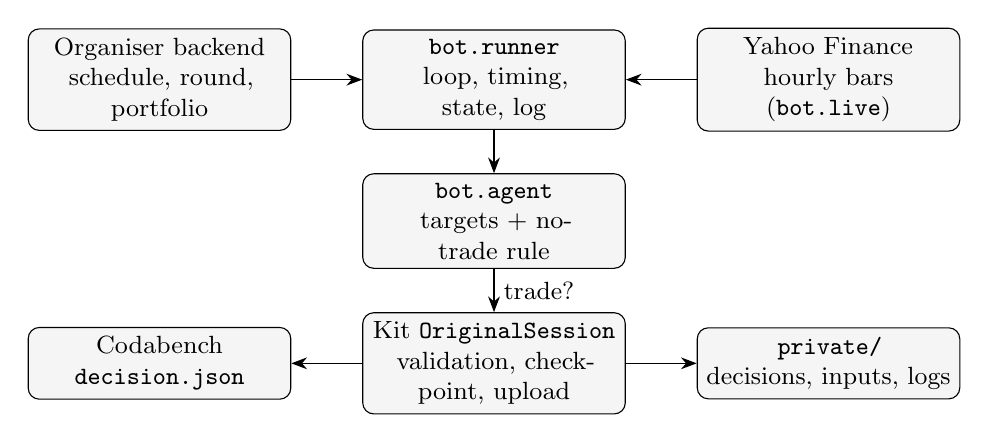
\begin{tikzpicture}[node distance=0.55cm and 0.9cm, every node/.style={font=\small},
  box/.style={draw, rounded corners, align=center, minimum height=0.9cm, text width=3.1cm, fill=gray!8},
  arr/.style={-{Stealth[length=2mm]}}]
\node[box] (sched) {Organiser backend\\schedule, round, portfolio};
\node[box, right=of sched] (runner) {\code{bot.runner}\\loop, timing, state, log};
\node[box, right=of runner] (yahoo) {Yahoo Finance\\hourly bars (\code{bot.live})};
\node[box, below=of runner] (agent) {\code{bot.agent}\\targets + no-trade rule};
\node[box, below=of agent] (kit) {Kit \code{OriginalSession}\\validation, checkpoint, upload};
\node[box, left=of kit] (cb) {Codabench\\\code{decision.json}};
\node[box, right=of kit] (arch) {\code{private/}\\decisions, inputs, logs};
\draw[arr] (sched) -- (runner);
\draw[arr] (yahoo) -- (runner);
\draw[arr] (runner) -- (agent);
\draw[arr] (agent) -- node[right]{trade?} (kit);
\draw[arr] (kit) -- (cb);
\draw[arr] (kit) -- (arch);
\end{tikzpicture}
\caption{Live architecture. All platform calls go through the starter kit's own client.}
\end{figure}

The runner (\code{python -m bot.runner --phase validation|official}) replaces the kit's \code{watch} command, which
cannot skip a round, stops entirely if the strategy raises, and holds the checkpoint lock for its whole lifetime. The
runner opens a kit session only for each platform interaction, so the kit's other commands remain usable while it runs.

\begin{algorithm}[h]
\small
\caption{Runner loop for one phase}
\While{phase not complete}{
  read schedule (server clock is authoritative)\;
  \If{a round $k$ is open and not yet handled}{
    wait until $o_k+3$ min\;
    \lIf{a decision file for $k$ exists}{re-upload it verbatim (resume) and stop}
    \lIf{the round already has an eligible attempt}{mark \emph{occupied}}
    read portfolio\;
    fetch and validate bars; retry every 2 min until deadline $-$ 10 min, else mark \emph{skipped} (hold)\;
    compute targets (approach 1 traded; 2 and 4 logged) and the no-trade rule\;
    \lIf{no trade}{mark \emph{held}; upload nothing}
    \Else{write \code{decision.json} and \code{inputs.parquet}; upload through \code{OriginalSession.decision}; mark \emph{submitted}}
    append a log record; persist state\;
  }
  sleep until the next window opens (at most 5 min)\;
}
\end{algorithm}

\paragraph{Data validation.} A download is rejected (and retried) if any symbol is missing or has a non-positive price.
It is also rejected if the last bar ends before the latest bar end $\hat e(t)$ that Yahoo should have published.
$\hat e(t)$ is the latest of today's 10:30, \dots, 15:30, 16:00 boundaries at or before $t-2$ min on weekdays,
otherwise the previous weekday's 16:00. On a market holiday this check fails safe (the round is skipped and the
portfolio held). Up to three symbols may miss only the latest bar, because Yahoo occasionally publishes a final bar late;
this was observed for TMO on 6 October 2026. Their previous close is carried forward and they are listed in the log.

\paragraph{Failure handling.}
\begin{center}\small
\begin{tabularx}{\linewidth}{lX}
\toprule
Situation & Behaviour \\
\midrule
Data stale or missing until the deadline & round skipped; holdings kept; no fee \\
Exception inside the agent & round skipped; loop continues \\
Platform error before the decision file exists & retried at the next poll (5 min) \\
Interrupted upload after the file exists & the identical bytes are resubmitted; the kit checkpoint reconciles by SHA-256 and never creates a duplicate \\
Ambiguous creation that the kit cannot reconcile & no automatic retry (kit policy); logged as \emph{error}, then \emph{missed} after the deadline \\
Slot already used & marked \emph{occupied}; nothing uploaded \\
Backend positions in an unknown format & falls back to the backend weight snapshot; if that is empty, the round is skipped rather than mistaking holdings for cash \\
\bottomrule
\end{tabularx}
\end{center}

\paragraph{Audit trail.} Every round appends one JSON line to \code{private/logs/decisions.jsonl} containing the code
version (git commit), the data diagnostics, the current weights and how they were obtained, all three targets
(approach~1, 2, 4), the expert weights, the deviation, the decision and the platform receipt. The team token is never
logged. For every submitted round the exact uploaded \code{decision.json} and the bar panel the agent saw
(\code{inputs.parquet}) are archived under \code{private/decisions/<phase>/<round>/}.

%=====================================================================
\section{Verification}\label{sec:tests}
%=====================================================================

The suite (\code{python -m pytest tests}, 65 tests, about 5 seconds) runs on synthetic data and a fake platform, so it
needs neither credentials nor network:
\begin{itemize}[nosep]
  \item \textbf{Constraints:} every construction respects stock and sector caps and its total, for random covariance
        matrices. Quantised weights always pass the kit's \code{\_weights} validator, including NaN inputs.
  \item \textbf{No lookahead:} features are invariant to truncation of the history. Multiplying all prices after a
        cutoff by random factors leaves every target at that cutoff unchanged, both live-style and in the backtester.
  \item \textbf{Accounting:} simulator metrics equal the kit's decimal reference calculator. Initial-allocation fee and
        turnover are exact. An all-cash strategy has zero return, drawdown and turnover.
  \item \textbf{End-to-end:} an in-memory Codabench and backend (\code{httpx.MockTransport}) drives the real kit
        client. Tests check one valid upload per round, holds within bands, skips on data or agent failure, respect for
        occupied slots, that a dry run never uploads, verbatim resume of an existing decision file, no duplicate after an
        ambiguous upload failure, and a complete simulated trading day (one trade, six holds, phase completion).
  \item \textbf{Replay:} a submitted decision is recomputed bit-for-bit from its archived inputs (\code{bot.replay}).
\end{itemize}
In addition, a dry run against the live organiser API (read-only) on 6 October 2026 produced a decision for
\code{validation-2026-10-08-r1} that the kit validator accepted for an upload time inside that round's window.

%=====================================================================
\section{Reproduction guide}\label{sec:repro}
%=====================================================================

\subsection{Environment}
Linux (tested on kernel 5.15), Python 3.13.2. Exact package versions are pinned in \code{requirements-bot.txt}:
lightgbm 4.7.0, numpy 2.5.3, pandas 3.0.6, pyarrow 25.0.1, scikit-learn 1.9.1, scipy 1.18.1, yfinance 1.7.0, httpx
0.28.1, pytest 9.1.1. No GPU is needed. The full experiment study takes about 12 minutes on 20 CPU cores; model
training takes about 10 seconds.

\subsection{Steps}
All commands run from the \code{starter-kit} directory.
\begin{enumerate}[leftmargin=1.4em]
\item \textbf{Install.}
\begin{lstlisting}
python3.13 -m venv .venv && . .venv/bin/activate
pip install -r requirements-bot.txt
cp .env.example .env && chmod 600 .env
# in .env: CODABENCH_TOKEN=<personal token>
#          ICAIF_PROFILE=profiles/profile99-production.json
\end{lstlisting}
\item \textbf{Build the data} (downloads dataset 1833, verifies its SHA-256, cleans it, downloads Yahoo data, writes
\code{private/data/data\_report.json}).
\begin{lstlisting}
python -m bot.data --refresh
\end{lstlisting}
\item \textbf{Run the tests.}
\begin{lstlisting}
python -m pytest tests
\end{lstlisting}
\item \textbf{Reproduce the study and the model.} The first command runs the 96-configuration grid and reports the grid
winner. The second evaluates overlays and robustness on the production core recorded in \code{bot/production.json}
(field \code{selected\_by}). Both commands train the walk-forward models and save the production model to
\code{bot/models/lgbm.txt} with metadata \code{lgbm.json}.
\begin{lstlisting}
python -m bot.experiments
python -m bot.experiments --core '{"core": "equal_weight|cap0.1|vt0.1|ex0.8|lb126|blend0.0", "band": {"band_l1": 0.2, "band_max": 0.05}, "target": "base", "alpha": null, "online": null}'
sha256sum bot/models/lgbm.txt
# expected: 0fe5e29dca33147f92af90df10de88eb
#           6eaef4b67007836d388ec8895fc3650e
\end{lstlisting}
Outputs go to \code{private/results/}: a summary (\code{experiments.json}) and one CSV file of per-window results for
each stage. Every table in this document was produced from these files.
\item \textbf{Check a live decision without uploading.}
\begin{lstlisting}
python -m bot.runner --phase validation --dry-run --simulate-round validation-2026-10-08-r1
\end{lstlisting}
\item \textbf{Trade a phase.} The runner is meant to run unattended; a systemd user unit is provided in \code{deploy/}.
\begin{lstlisting}
python -m bot.runner --phase validation
python -m bot.runner --phase official
\end{lstlisting}
\item \textbf{Regenerate a submitted decision} from its archived inputs and logged portfolio. The command exits with
status 0 only if the recomputed weights equal the uploaded ones exactly.
\begin{lstlisting}
python -m bot.replay private/decisions/official/official-2026-10-12-r1
\end{lstlisting}
\end{enumerate}

\subsection{Determinism}
\begin{itemize}[nosep]
  \item The official dataset is fixed by checksum. Cleaning is deterministic.
  \item LightGBM runs with \code{deterministic=true}, a fixed seed and a fixed thread count. Retraining on 6 October 2026
        reproduced the stored model byte for byte (same SHA-256). The production decision does not use the model.
  \item The competitor field is generated with a fixed seed (\code{seed=11}).
  \item Yahoo data is not under our control: Yahoo may revise bars and keeps only about 730 days of hourly history.
        Experiments on Yahoo data are therefore reproducible to within such revisions. Live decisions are reproducible
        exactly from the archived \code{inputs.parquet} files.
  \item The production decision depends only on the bar history, the backend portfolio and \code{production.json}. The
        shadow targets also depend on the online expert state, which is stored in \code{private/state/runner\_<phase>.json}
        and logged every round.
\end{itemize}

\subsection{Code map}
\begin{center}\small
\begin{tabularx}{\linewidth}{lX}
\toprule
Path & Role \\
\midrule
\code{bot/data.py} & dataset download, checksum, cleaning, spinoff adjustment, Yahoo cache, cross-checks \\
\code{bot/market.py} & bar panels, bar end times, round timeline, execution prices \\
\code{bot/features.py} & 31 causal features \\
\code{bot/risk.py} & covariance estimators, portfolio constructions, cap enforcement \\
\code{bot/agent.py} & approaches 1, 2 and 4; configuration; no-trade rule \\
\code{bot/alpha.py} & LightGBM dataset, training, purged walk-forward, IC \\
\code{bot/backtest.py} & competition simulator, windows, competitor field, rank scoring \\
\code{bot/experiments.py} & the full study and model export \\
\code{bot/live.py} & live Yahoo download, freshness checks, portfolio parsing \\
\code{bot/runner.py} & live loop and uploads through the kit client \\
\code{bot/replay.py} & bit-exact regeneration of submitted decisions \\
\code{bot/production.json} & production configuration \\
\code{bot/models/lgbm.\{txt,json\}} & production LightGBM model and metadata \\
\code{tests/} & 65 automated tests \\
\code{deploy/icaif-runner@.service} & optional systemd user unit \\
\bottomrule
\end{tabularx}
\end{center}

%=====================================================================
\section{Limitations}
%=====================================================================
\begin{itemize}[nosep]
  \item \textbf{Invented field.} The rank-based results depend on a field of competitors we constructed. Real teams may
        be stronger or weaker on return, which changes the optimal exposure (Proposition~\ref{prop:scaling}). This is why
        we report the sensible sub-field as well and chose $e_{\max}=0.8$ over the marginally better 0.6.
  \item \textbf{Fee convention.} The backend's exact fee sizing is unpublished; the effect is second order.
  \item \textbf{Execution prices on official data} are approximated by bar midpoints for 10:30--15:30. The Yahoo
        backtest uses exact bar opens.
  \item \textbf{Short horizon.} A 15-day phase is short. Even a sound strategy can finish poorly in a given window; the
        worst historical window lost 8.6\% with a 13.4\% drawdown.
  \item \textbf{Portfolio format.} The backend's position schema was unknown until the first Validation execution. The
        parser accepts the common forms and fails safe.
  \item \textbf{Data provider.} The agent depends on Yahoo Finance availability. Outages lead to held rounds, not to
        erroneous trades.
\end{itemize}

\end{document}
